\documentclass[a4paper,12pt]{article}
\usepackage{titling}
\usepackage{lscape}
\usepackage{amssymb, amsmath, amssymb}
\usepackage{booktabs}
\usepackage{makecell}
\usepackage{float}
\floatplacement{figure}{H}
\usepackage[stable]{footmisc}
\usepackage{lmodern}
\usepackage{microtype}
\usepackage{libertine}
\usepackage[libertine]{newtxmath}
\usepackage[scale=.8]{FiraMono}
\usepackage[usenames, dvipsnames]{xcolor}
\usepackage{setspace}
\usepackage{float}
\usepackage[top=2cm, bottom=2cm, left=2cm, right=2cm]{geometry}
\usepackage{graphicx}
\usepackage{xcolor}
\definecolor{darkblue}{rgb}{0.0,0.0,0.55}
\usepackage{dcolumn}
\usepackage{mathtools}
\usepackage{caption}
\usepackage[UKenglish]{babel}
\usepackage[UKenglish]{isodate}
\usepackage[authoryear]{natbib}
\usepackage{babelbib}
\cleanlookdateon
\exhyphenpenalty=10000
\hyphenpenalty=10000
\widowpenalty=10000
\clubpenalty=10000
\setcitestyle{aysep={}} 
\usepackage{etoolbox}
\makeatletter
\patchcmd{\NAT@citex}
	  {\@citea\NAT@hyper@{%
		 \NAT@nmfmt{\NAT@nm}%
		 \hyper@natlinkbreak{\NAT@aysep\NAT@spacechar}{\@citeb\@extra@b@citeb}%
		 \NAT@date}}
	  {\@citea\NAT@nmfmt{\NAT@nm}%
	   \NAT@aysep\NAT@spacechar\NAT@hyper@{\NAT@date}}{}{}
	\patchcmd{\NAT@citex}
	  {\@citea\NAT@hyper@{%
		 \NAT@nmfmt{\NAT@nm}%
		 \hyper@natlinkbreak{\NAT@spacechar\NAT@@open\if*#1*\else#1\NAT@spacechar\fi}%
		   {\@citeb\@extra@b@citeb}%
		 \NAT@date}}
	  {\@citea\NAT@nmfmt{\NAT@nm}%
	   \NAT@spacechar\NAT@@open\if*#1*\else#1\NAT@spacechar\fi\NAT@hyper@{\NAT@date}}
	  {}{}
\makeatother
\usepackage[hyphens]{url}
\usepackage[hidelinks]{hyperref}

\hypersetup{
	pdftitle={Do Elites Support Polycentric Climate Governance?},
	pdfauthor={Danilo Freire, Umberto Mignozzetti, and David Skarbek},
	pdfsubject={Climate change governance},
    pdfkeywords={climate change, conjoint experiment, elites, Latin America, polycentrism},
	pdfborder={0 0 0},
	breaklinks=true,
	linkcolor=Mahogany,
	citecolor=Mahogany,
	urlcolor=darkblue,
	colorlinks=true} %

\doublespacing

\title{Do Elites Support Polycentric Climate Governance? Evidence from Ten Latin American Countries\thanks{We thank Nigel Ashford, F\'{a}bio Barros, Daniel D'Amico, Malte Hendricks, Christian H\"{u}bner, Karina Marzano, Emily Skarbek, and Matias Spektor for helpful and engaging feedback. This research received financial support from the Konrad Adenauer Stiftung Latin American Regional Programme for Energy Security and Climate (EKLA-KAS). The authors declare there are no conflicts of interest. The data, code, and any additional materials required to replicate all analyses in this article are available at \href{http://github.com/danilofreire/climate-governance}{\texttt{http://github.com/danilofreire/climate-governance}}.}}

\author{Danilo Freire\thanks{Postdoctoral Research Associate, The Political Theory Project, Brown University, Providence, RI 02912, USA, \href{mailto:danilo_freire@brown.edu}{\texttt{danilo\_freire@brown.edu}}, \href{http://danilofreire.github.io}{\texttt{http://danilofreire.github.io}}, \href{http://twitter.com/danilofreire}{\texttt{http://twitter.com/danilofreire}}, Voice: +1 (401) 584-2494. Corresponding author.} 
\and Umberto Mignozzetti\thanks{School of International Relations, Funda\c{c}\~{a}o Getulio Vargas, S\~{a}o Paulo, SP, Brazil and Wilf Family Department of Politics, NYU, NY, USA, \href{mailto:umberto.mig@nyu.edu}{\texttt{umberto.mig@nyu.edu}}, \href{http://umbertomig.com}{\texttt{http://umbertomig.com}}, \href{http://twitter.com/umbertomig}{\texttt{http://twitter.com/umbertomig}}.} \and David Skarbek\thanks{The Department of Political Science and the Political Theory Project, Brown University, Providence, RI, USA, \href{mailto:david_skarbek@brown.edu}{\texttt{david\_skarbek@brown.edu}}, \href{http://davidskarbek.com}{\texttt{http://davidskarbek.com}}, \href{http://twitter.com/davidskarbek}{\texttt{http://twitter.com/davidskarbek}}.}
}

\date{\today}

\begin{document}
\maketitle

\begin{abstract}
\onehalfspacing
\noindent
Policy makers generally assume that climate change mitigation requires global scale governance. In contrast, recent studies suggest that polycentrism provides an effective alternative to top-down environmental policies. But despite the high social costs each solution implies, it is unclear which institutional arrangement potential veto players support. Here we run a conjoint experiment with elite members of 10 Latin American countries and ask respondents to evaluate 6,000 possible climate change agreements. We find that institutional features have a substantial effect on support for climate treaties. Latin American elites prefer multilevel state-based solutions to global warming, but there is considerable heterogeneity across countries and elite types. Our results suggest novel ways to craft accountable, democratic climate change mitigation agreements, and they offer new insights on how to integrate interventions at the local and international levels.

\vspace{.5cm}

\noindent 
\textbf{Keywords:} climate change, conjoint experiment, elites, Latin America, polycentrism

\vspace{.5cm}

\noindent 
\textbf{Word count:} 3,000
\end{abstract}

\newpage

\doublespacing

\section{Introduction}%
\label{sec:introduction}

Over the last years, we have seen an emerging consensus about the causes and consequences of anthropogenic climate change. Despite some variation in climate risk beliefs, mostly due to cultural worldviews and political orientation \citep{hornsey2016meta}, recent surveys show that the public is increasingly aware of the dangers of greenhouse gas emissions. For example, 59\% of Americans are sure the Earth's temperature is increasing \citep{stanfordearth2018}; 74\% of European Union citizens consider global warming a `very serious problem' \citep{europe2018survey}; and 90\% of Brazilians believe climate change is already harming people around the world \citep{pew2018climate}.

Yet this consensus does not translate itself into effective political action. Global climate negotiations have progressed slowly under the guidelines of the United Nations Framework Convention on Climate Change (UNFCCC), and there is wide scepticism that multilateral talks will move faster in the next years \citep{cole2015advantages, hjerpe2015views}. As carbon dioxide emissions continue to increase, current efforts are likely to be insufficient to meet the Paris Agreement target of $2^{\circ}$C temperature rise above pre-industrial levels \citep{jordan2015emergence}. Existing research affirms that this unsatisfactory performance is partially due to institutional design \citep{ostrom2014polycentric, cole2015advantages}. For instance, multilateral forums downplay the domestic constraints political leaders experience when implementing strategies to reduce greenhouse gas emissions \citep{rayner2010eat}. Universal binding agreements also offer limited scope for experimentation, which hinders the ability for individuals to solve complex collective action problems \citep{de2014global}.

Recently, scholars have argued that polycentric approaches provide a better `institutional fit' for natural resource systems \citep{turnheim2018innovating,berkhout2003negotiating, carlisle2017polycentric, ostrom1990governing}. Polycentrism is defined as a political arrangement in which formally independent units operating at different levels engage in a continuous process of cooperation and competition \citep{cole2015advantages,aligica2013co}. Experiences such as inshore fisheries in Turkey and timber management in Switzerland show that polycentrism induces individual cooperation and allows communities to avoid the `tragedy of the commons', that is, the overexploitation of shared resources \citep{hardin1968tragedy, ostrom1990governing}. Authors also point out that polycentric systems improve accountability as decentralisation reduces rent-seeking opportunities for politicians and interest groups \citep{turnheim2018innovating,ostrom2012nested,ostrom2014polycentric,sovacool2013adaptation}. 

Despite the potential advantages of polycentric arrangements, two challenges may undermine their popular support. First, polycentric systems demand constant civic participation at multiple government levels. But as climate change has diffuse benefits but concentrated costs, individuals have few incentives to join collective efforts \citep{barrett2003increasing, heitzig2011self, nordhaus2015climate}. Second, individuals tend to heavily discount climate change investments \citep{dasgupta2008discounting, nordhaus1997discounting}. Reducing carbon emissions requires significant expenditures today, yet the benefits of climate mitigation will arise only in a distant future. In that regard, citizens might prefer state-based initiatives to prevent climate change if private costs are too high or expected results too uncertain. 

Voluntary environmental governance faces further difficulties in new democracies. In Latin America, authoritarian regimes discouraged civil participation and reduced social capital, two necessary conditions for effective polycentric arrangements \citep{aligica2014institutional,ostrom1990governing}. Top-down climate policies also create incentives for organised groups to collude with state officials and pursue private interests. As a result, elites and state representatives have \textit{de facto} veto power over environmental legislation and can override local decisions to their own benefit.

We design a conjoint experiment to assess which climate change governance system Latin American elites are willing to support. In our survey, we asked 654 `elites' -- academics, members of the executive power, legislators, businesspeople, and members of non-governmental organisations -- to select their preferred agreement in 7 randomised binary choices. We recruited respondents from Argentina, Brazil, Bolivia, Chile, Colombia, Costa Rica, Ecuador, Mexico, Panama, and Peru.

In what follows, we describe our experimental methods and results. We then turn to two additional analyses, in which we disaggregate the responses according to country and elite type, and proceed to the concluding remarks.

\section{Data and Methods}%
\label{sec:data_and_methods}

We use a conjoint experiment to analyse how institutional characteristics shape support for climate change agreements in Latin America. First, Latin America is the most biodiverse region in the world and it plays a major role in global climate mitigation projects. For instance, the Amazon basin contains about half of the world's carbon stock, so local elites are essential for the success of emissions trading markets \citep{yang2018post}. Second, Latin American elites have wide disagreements over preservations policies, and the recent shift towards populist governments has highlighted the need for a robust framework to protect environmental resources \citep{ellner2019pinktide}. In that regard, veto players can counterbalance governmental time discounting and secure the long-term provision of public goods. Lastly, survey experiments on climate policies have focused on a small set of developed countries, so truly comparative experimental work remains scarce. We fill this gap by analysing 10 countries where elites have different stakes at climate change negotiations.  

We use a dataset compiled specifically for this study. From 1\textsuperscript{st} of October to 5\textsuperscript{th} of December 2018, we ran an elite survey in ten Latin American countries: Argentina, Bolivia, Brazil, Chile, Colombia, Costa Rica, Ecuador, Mexico, Panama, and Peru. We started by collecting information on Latin American elites. Our target was to interview 10 members of the Executive, 10 members of the Legislative, 15 academics, and 15 members of the civil society per country. To do so, we built a dataset of prospective respondents ten times our country target. Then, we ran an online and telephone survey where we collected information regarding the climate change agreements and other related questions.

After finishing this dataset, we started the surveying stage. From 12\textsuperscript{th} of November to 5\textsuperscript{th} of December, we ran the survey by contacting elite members by phone or by email. We had two teams of enumerators, one based in S\~{a}o Paulo and another based in Rio de Janeiro, Brazil, comprised of Portuguese and Spanish native speakers. Although the overall aim of the survey was 500 responses, the teams collected 654 interviews. Please refer to the Supplementary Material for more information about the sampling process and descriptive statistics.

The hypothetical climate change agreements includes six attributes: 1) which organisation defines the rules; 2) how would conflicts be resolved; 3) what punishment should be applied to rule-breakers; 4) how should repeated violations be sanctioned; 5) which countries should bear the costs of the agreement; 6) how often should the agreement be renegotiated. Table~\ref{tab:categories} describes the values we included in each treaty attribute. \\

\newpage 

\begin{table}[ht]
\begin{center}
\caption{\textbf{Design principles for climate change mitigation conjoint experiments}}
\label{tab:categories} 
\begin{tabular}{l !{\vrule width 1pt}p{9cm}}
\Xhline{2\arrayrulewidth}
\textbf{Attribute} & \multicolumn{1}{c}{\textbf{Values}} \\
\Xhline{2\arrayrulewidth} \\
Who makes the rules? & International organisations; federal government; local government; local community members; non-governmental organisations \\
& \\
Conflict resolution mechanism & United Nations; government bureaucracy; local courts; private arbitration; informal norms \\
& \\
Punishment & Imprisonment; fines; blacklist; none \\
& \\
Punishment for repeated violations & More penalty; same; less penalty \\
& \\
Agreement costs & Rich countries pay more than poor countries; proportional to history of emissions; proportional to current emissions; only rich countries pay \\
& \\
Renegotiation & Never; fifty years; twenty years; five years; one year \\
\Xhline{2\arrayrulewidth} 
\end{tabular}
\end{center}
\end{table}

The categories map the main conceptual differences between polycentric and state-led climate mitigation policies \citep{bechtel2013mass, ostrom1990governing}. The conjoint experiment design open the possibility for respondents to combine multiple levels of governance into a single climate change agreement as they see fit. We give no prior indication of whether a certain value is more prevalent in actual agreements, and we randomise the values to ensure that they all have the same probability of being selected. In total, there are 6,000 possible value combinations. Figure~\ref{fig:conjoint} illustrates our experimental design.

\begin{figure}[H]
	\centering
	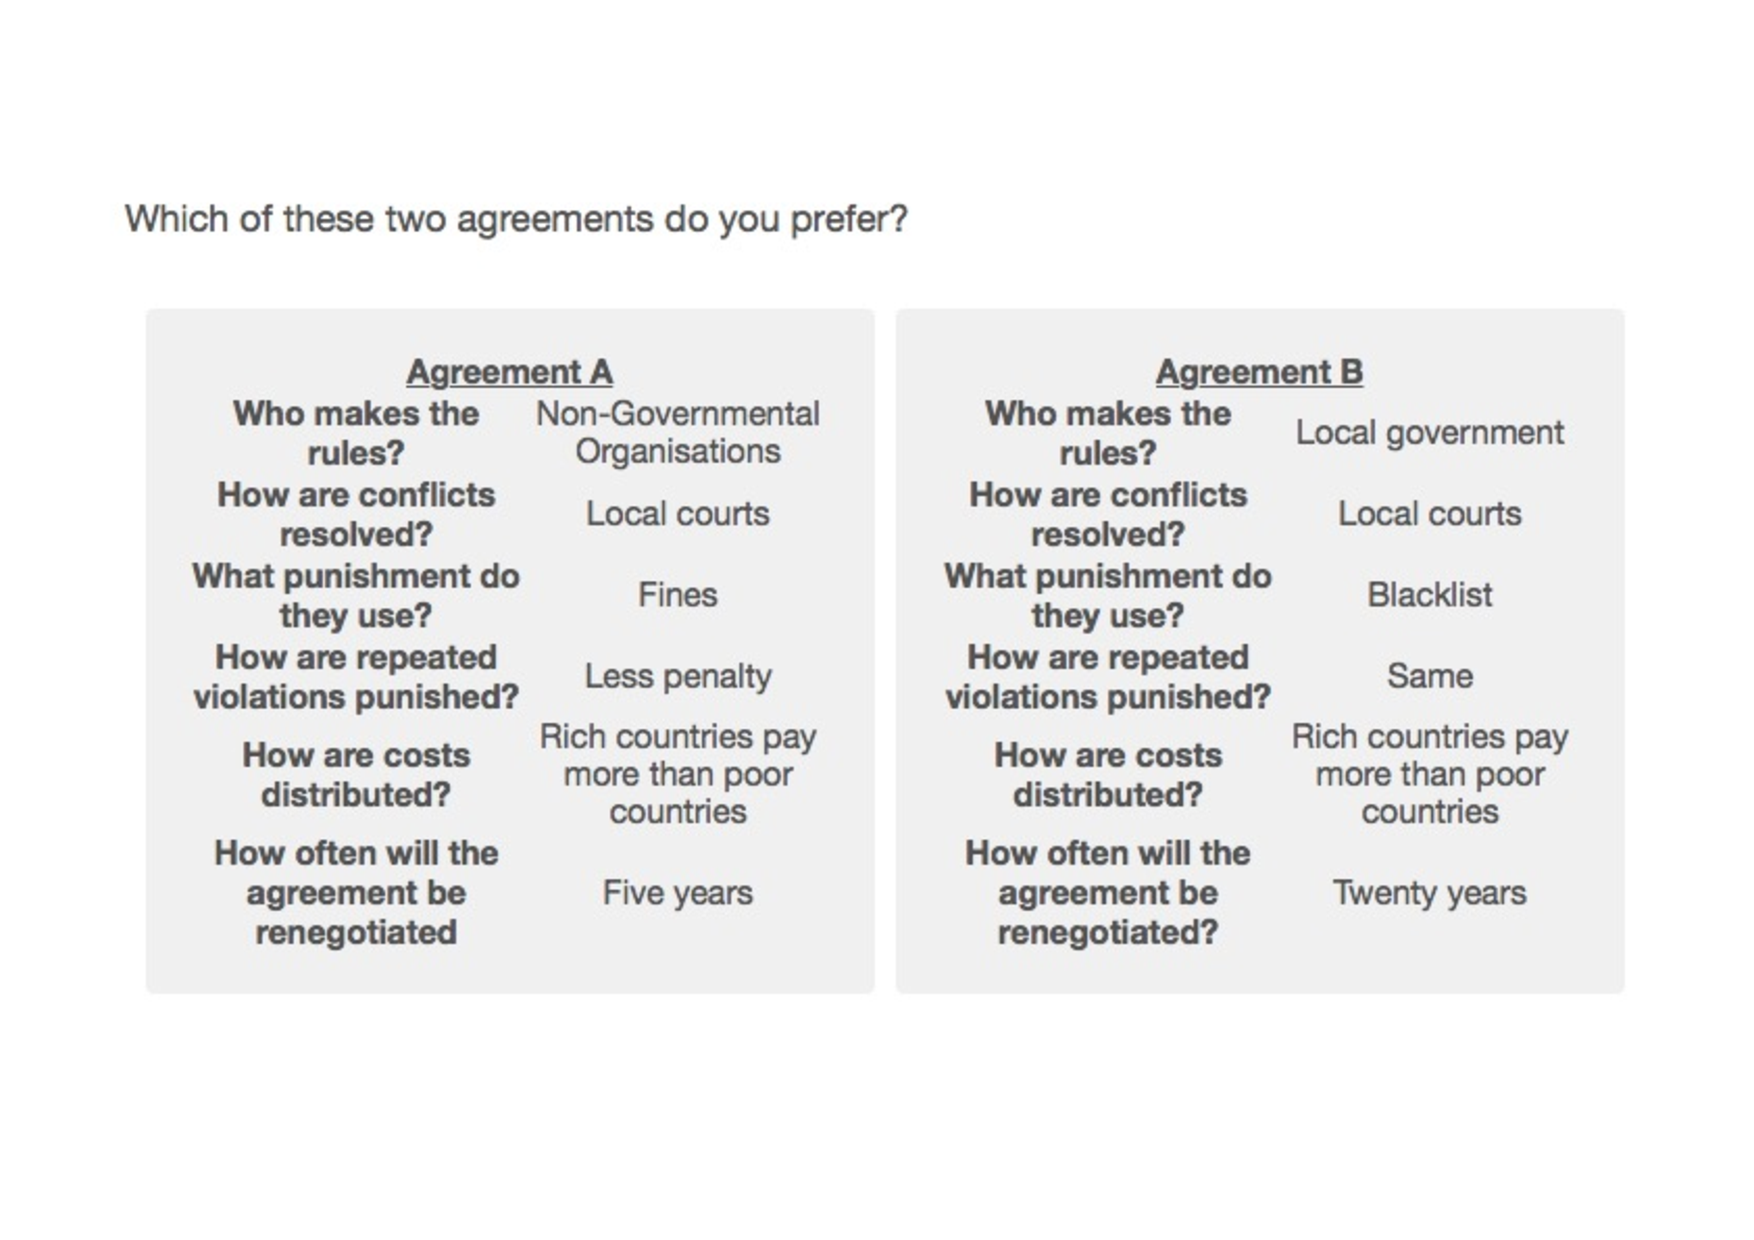
\includegraphics[width=13cm]{conjoint-cropped.pdf}
	\caption{\textbf{Example of conjoint experiment design}}
	\label{fig:conjoint}
\end{figure}

We estimate our models with the \texttt{cregg} package \citep{leeper2018cregg} for the \texttt{R} statistical language \citep{rstats2019}. We report marginal means instead of average marginal conditional effects (AMCE). \citet{leeper2018subgroup} show that AMCEs can be misleading when applied to subgroup analysis as results are sensitive to the choice of reference categories in interactions. Marginal means provide a clear description of quantities of interest -- preference towards a given attribute -- and allows for easy comparisons between different groups of respondents. AMCE estimates are available in the Supplementary Materials.

\section{Results}%
\label{sec:results}

Figure~\ref{fig:pooled} shows our main results. The findings indicate that Latin American elites have a strong preference for a polycentric approach to mitigate climate change. We see that the respondents have a positive view about two sources of climate governance, namely those located at the international and the local levels. Importantly, Latin American elites support both levels \textit{simultaneously}; this provides evidence that they favour agreements which incorporate action separate political spheres at the same time in the same regime. 

\begin{figure}[H]
	\centering
	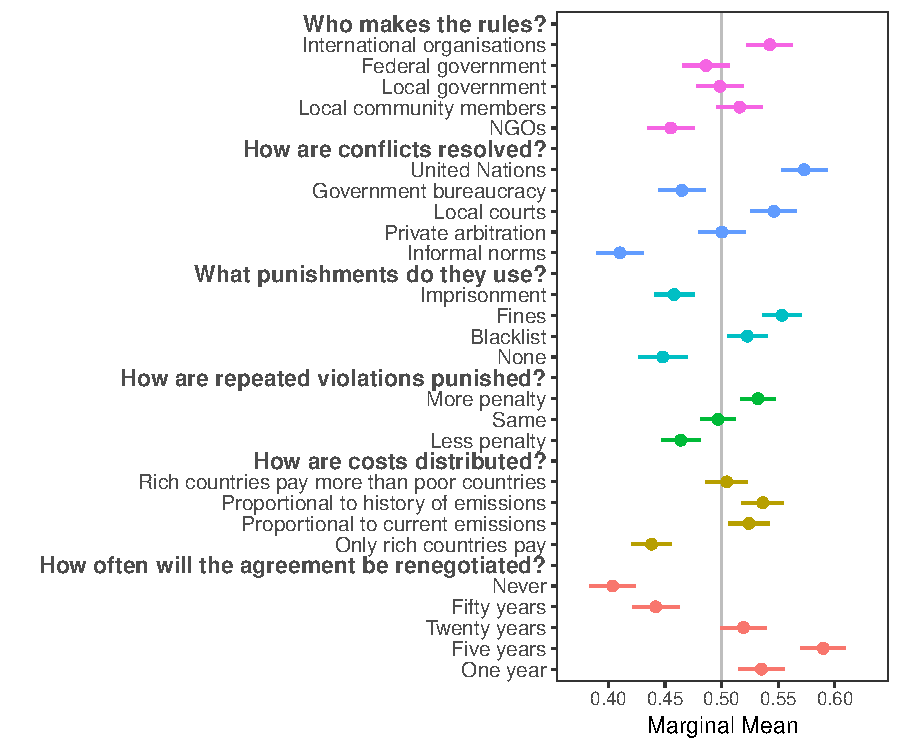
\includegraphics[width=.9\linewidth]{pooled.pdf}
	\caption{\textbf{Effect of agreement dimensions on the probability of support for climate change agreement in 10 Latin American countries (pooled data).} The horizontal bars correspond to the 95\% confidence interval of the estimated effect. Standard errors are clustered by respondent (respondents = 651; comparisons = 7,968). Full numerical estimates are available in the Supplementary Information Appendix.}
	\label{fig:pooled}
\end{figure}

Climate change agreements designed by international organisations are viewed more favourably than the alternatives. Global institutions receive 54\% (SE = 1.25) of acceptance in our sample. At the same time, respondents clearly indicate their preference for bottom-up rule-making. Agreements formulated by local community members and local governments are the second and third-preferred choices with 51.6\% (SE = 1.25) and 49.8\% (SE = 1.24) approval. In contrast, Latin American elites see non-governmental organisations are their least preferred option for climate change rule-making with 45.5\% (SE = 1.26). 

We see a similar pattern with respect to conflict resolution. Respondents suggest disputes should be addressed mainly by the United Nations and local courts. These two choices have 57.3\% (SE = 1.22) and 54.6\% (SE = 1.23) approval, respectively. Private arbitration comes next with 50\% (SE = 1.26), followed by government bureaucracy with 46.4\% (SE = 1.25). Informal norms is the least preferred mechanism to deal with conflicts between agreement parties (41\%, SE = 1.25). 

In line with Ostrom's predictions, Latin American elites agree with graduated sanctions to repeated offenders (53.2\%, SE = 0.94) and they believe agreement costs should be allocated according to the country's history of emissions (53.6\%, SE = 1.14). Moreover, related to the same idea of proportionality, respondents indicate that lawbreakers should be punished with fines (55.3\%, SE = 1.06), which can be easily increased if necessary.

We find no evidence that rich countries alone should bear the burden of climate change mitigation costs. Latin American elites believe developing countries should also contribute to the provision of global public goods. This suggests that elites view it was legitimate to contribute to climate change solutions, so this may not be a major source of free riding to climate change solutions in the region.

In terms of agreement duration, respondents are interested in a balance between stability and flexibility. This also lends support to Elinor Ostrom's theory of polycentric climate change governance. Agreements that either cannot be modified or that last for 50 years are rejected by the interviewees. Their preference lies in agreements that can be renegotiated every five years (59\%, SE = 1.2), as they are durable enough to provide long-term incentives to the parties, yet still adaptable to unforeseen demands.

We also examine if our results vary across countries and types of elites. Figure~\ref{fig:countries} displays the preferred climate change agreement characteristics for each of the 10 countries in our sample. Despite Latin America's wide social heterogeneity, we observe that the results are notably similar. Most respondents affirm that the United Nations should be responsible for resolving conflicts, and six of them place local courts as the second-preferred choice. Peruvian elites are the only to prefer private arbitration to mediate disputes (60.7\%, SE = 4.5). We see that respondents in eight out of ten countries are willing to apply fines as punishment for agreement violators, with Chileans and Ecuadorians stating they would rather blacklist defectors. The majority also prefers to employ more penalties to repeated offenders. 

Another interesting cross-country similarity is that our sample largely supports agreements that can be renegotiated every five or twenty years. The difference is particularly wide in Costa Rica, where five-year agreements receive 29.4\% more approval than treaties that will never be revised. Chileans, in contrast, have the largest gap between one-year and five-year agreements: 22.7\%. Two possible explanations is that Chilean elites are either sensitive to transaction costs of negotiating repeated agreements, or they worry that one-year treaties may not provide enough stability for collective action.

\begin{figure}[H]
	\centering
	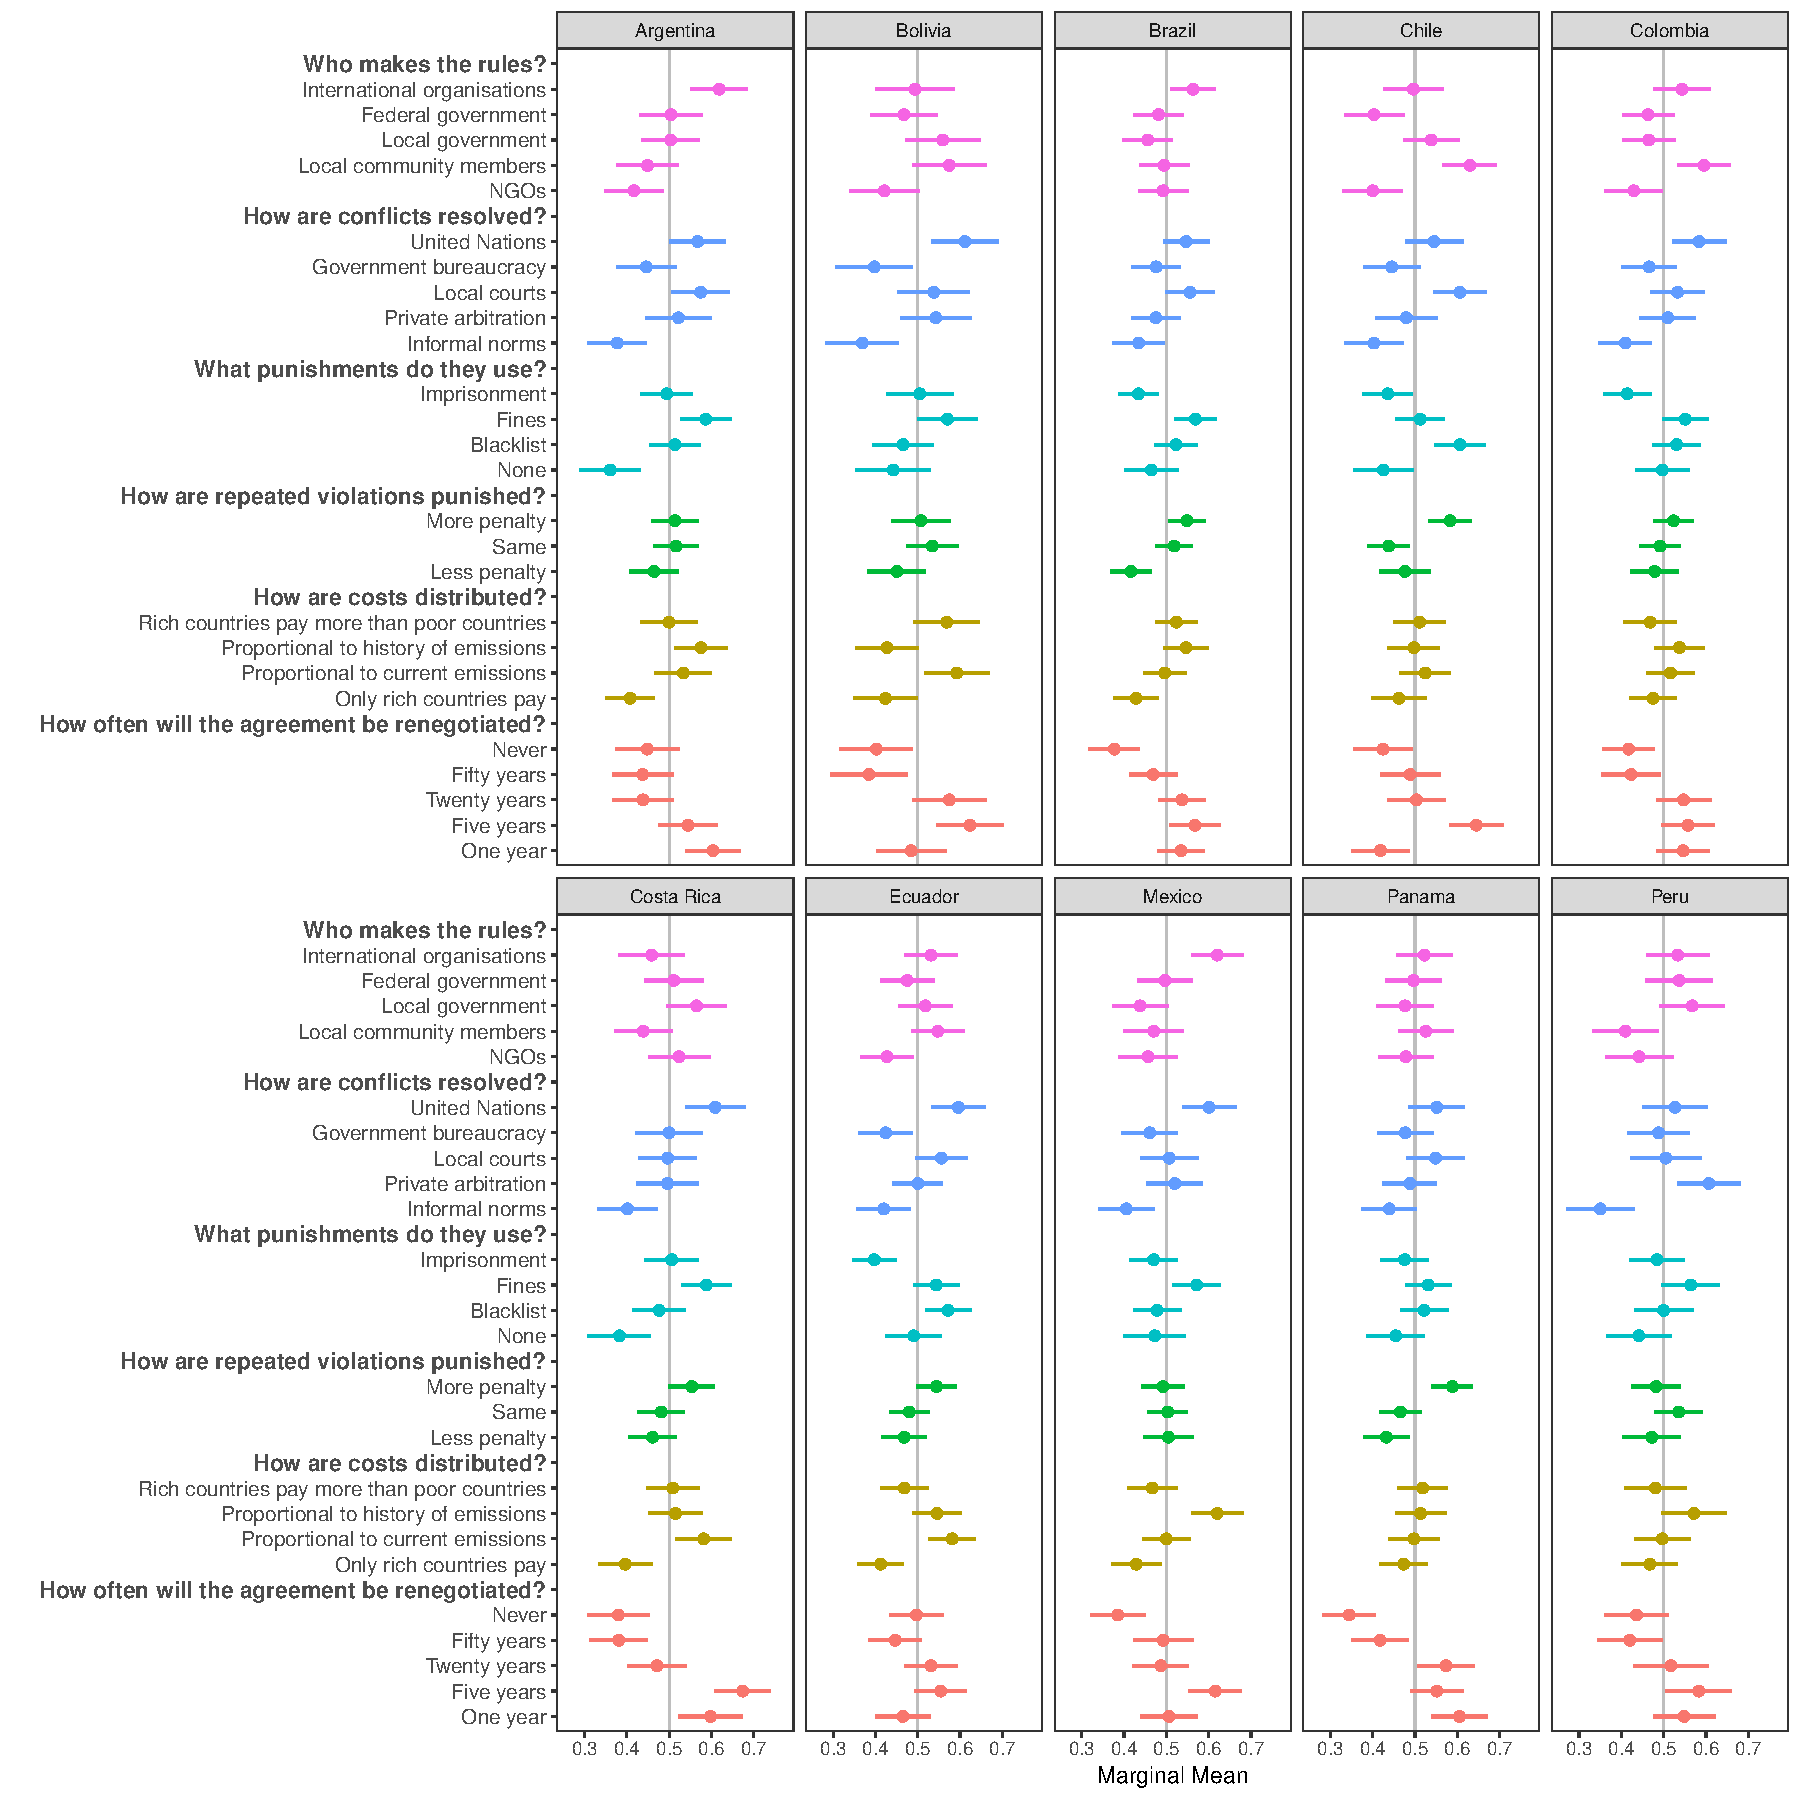
\includegraphics[width=\linewidth]{countries.pdf}
	\caption{\textbf{Effect of agreement dimensions on the probability of support for climate change agreement by country.} Bars represent 95\% confidence intervals.}
	\label{fig:countries}
\end{figure}

There are some interesting differences about which institutions should make the agreement rules. Argentinians are particularly sceptical about local community members (44.9\%, SE = 4.4) and favourable towards international organisations (61.9\%, SE = 4.1), whereas Bolivians believe local communities (57.5\%, SE = 5.3) and governments (55.9\%, SE = 5.4) are the best source for climate change rules. Respondents in most countries place NGOs as their least-preferred option, but elites from Brazil and Costa Rica have a more positive view of these organisations. Federal governments receive the lowest support in Chile, but respondents have the highest preference for local communities with 63\% (SE = 3.9). 

Figure~\ref{fig:types} shows the results disaggregated by elite type. We find that several positions are comparable across all subgroups. Academics, members of the civil society, and representatives in the executive and legislative branches hold similar views about how conflicts should be resolved, what punishment to apply to lawbreakers (fines and blacklisting), and the duration of the agreements.

\begin{figure}[H]
	\centering
	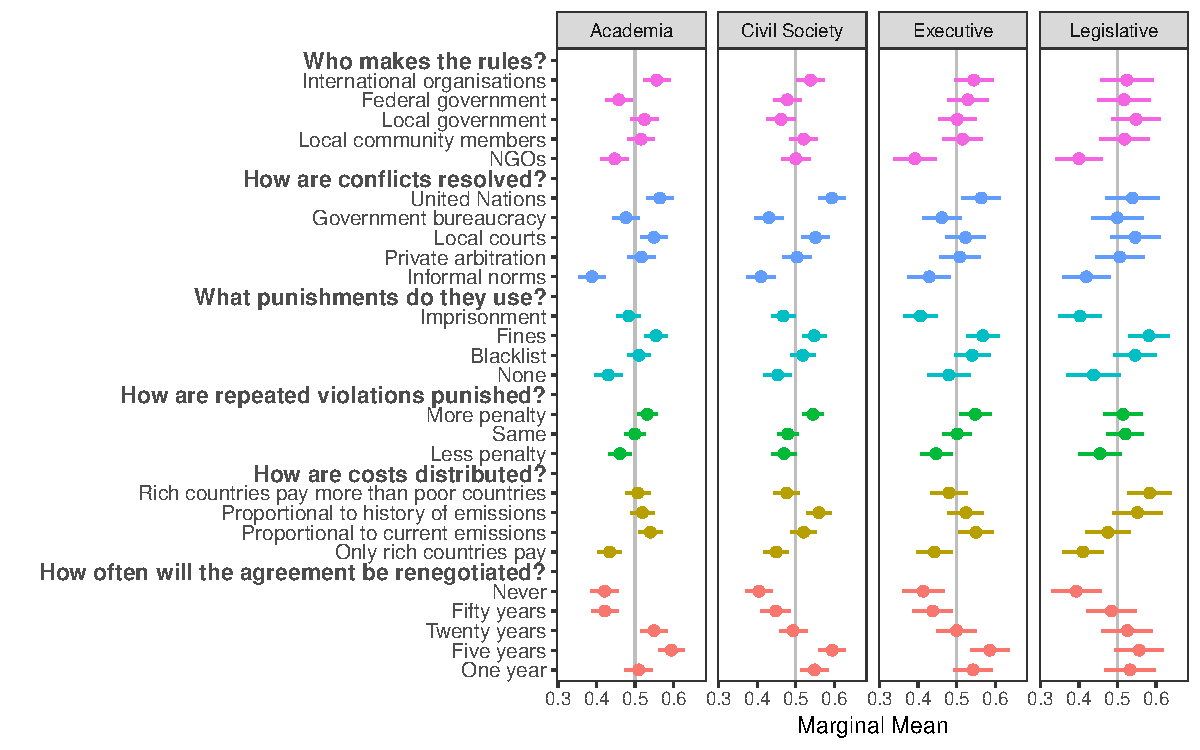
\includegraphics[width=\linewidth]{types.pdf}
	\caption{\textbf{Effect of agreement dimensions on the probability of support for climate change agreement by elite type.} Bars represent 95\% confidence intervals.}
	\label{fig:types}
\end{figure}

Differences emerge in two of the six dimensions of interest. First, whereas academics and members of the civil society are less favourable to allowing the federal government to formulate the rules, members of the executive and the legislative -- part of federal government themselves -- are more likely to see themselves as the preferred rule-makers. Second, members of the legislative have a stronger opinion that rich countries should bear the larger part of the agreement costs (58.4\%, SE = 3.5). 

\section{Discussion}
\label{sec:discussion}

In this article, we analyse whether Latin American elites support a polycentric climate change mitigation regime. We find that respondents prefer international organisations to create rules and resolve conflicts, to impose increasing fines on violators and to renew agreements every five years.  The results also suggest that respondents are sceptical about non-governmental organisations and consistently reject informal norms as an instrument to solve disputes. Taken together, our experiment is very consistent with the Latin American tradition of heavier reliance on the state than on voluntary solutions. After disaggregating the data by country and elite type, we find large heterogeneity in the responses. Nevertheless, elites remain sceptical about civil society organisations and informal norms. 

Our results have important theoretical and practical implications. The findings we present here suggest there is considerable scope for new studies on global governance, specially in underrepresented regions. Our analysis can be extended to examine if the Latin American public has the same opinion on multilevel arrangements as do the elites; and if not, it would be important to know what explains the mismatch between groups. Moreover, future work may address whether other areas of scholarship which assume international-level coordination could benefit from multilevel arrangements, either state-based or not.   

The findings also highlight the importance of comparative work in experimental studies. As a region, Latin America favours results that are in line with polycentric arrangements, but we find that those preferences derive from the aggregation of heterogeneous effects. Our study indicates researchers should be cautious about the external validity of experimental findings. % Add a couple more sentences here 

With regards to environmental policies, we provide experimental evidence that individuals have preferences that are not fully represented in current climate mitigation agreements. We identify that Latin American elites are interested in incorporating different political actors and in strengthening the role international organisations play in climate governance. Future climate negotiations can achieve better results if they take those preferences into account. 

\section*{Supplementary Material}
\label{sec:supplementary}

Please visit \href{http://github.com/danilofreire/climate-governance}{\texttt{http://github.com/danilofreire/climate-governance}} for supplementary materials for this article.

\newpage

\bibliographystyle{apalike}
\bibliography{references.bib}

\end{document}

